\begin{titlepage}
    \begin{center}
        \fontsize{14pt}{12px}\selectfont
        \textbf{POLITECHNIKA WARSZAWSKA} \\
        WYDZIAŁ ELEKTRYCZNY \\
        INSTYTUT STEROWANIA I ELEKTRONIKI PRZEMYSŁOWEJ

        \vspace*{.6\baselineskip}

        \fontseries{b}\fontsize{12pt}{10pt}\selectfont
        PRACA DYPLOMOWA MAGISTERSKA \\
        na kierunku INFORMATYKA \\
        specjalność: inżynieria oprogramowania
    \end{center}

    \begin{flushleft}
        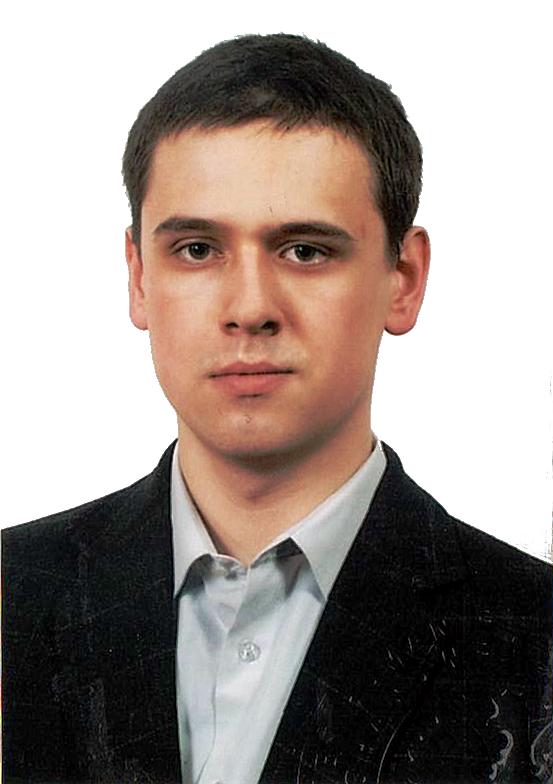
\includegraphics[width=4cm]{img/zdjecie_dyplo.png} \\
        \fontsize{14pt}{12px}\selectfont
        Jakub SAŁKOWSKI \\
        \fontseries{b}\fontsize{12pt}{10pt}\selectfont
        Nr albumu: 248418
    \end{flushleft}

    \begin{flushright}
        \begin{minipage}{0.3\textwidth}
            \fontsize{12pt}{10pt}\selectfont
            Rok akad.: 20013/2014 \\		
            \fontsize{10pt}{8pt}\selectfont
            Warszawa, \textit{2013.05.12}
        \end{minipage}
    \end{flushright}

    \vspace*{1\baselineskip}

    \begin{center}
        \fontseries{b}\fontsize{14pt}{12pt}\selectfont
        PROJEKT I~REALIZACJA APLIKACJI ODCZYTUJĄCEJ NUMERY
        AUTOBUSÓW NA URZĄDZENIA MOBILNE Z SYSTEMEM ANDROID
    \end{center}

    \vspace*{1\baselineskip}

    \begin{flushleft}
        \fontseries{b}\fontsize{12pt}{10pt}\selectfont
        Zakres pracy:
        \fontseries{m}\fontshape{it}\selectfont
        \begin{enumerate}
            \item Wprowadzenie i~sformułowanie celu pracy
            \item Przegląd metod detekcji
                i~identyfikacji obiektów w obrazach
            \item Przygotowanie środowiska wspomagającego
                implementację i~weryfikację algorytmów
            \item Analiza porównawcza wybranych
                metod detekcji i~identyfikacji obiektów w~obrazach
            \item Implementacja i~weryfikacja najbardziej efektywnego algorytmu
                na kilku urządzeniach z~systemem Android
            \item Wnioski i~podsumowanie
        \end{enumerate}
        \fontshape{n}\fontseries{b}
        \fontsize{12pt}{10pt}\selectfont

        \vspace*{1\baselineskip}

        Kierujący pracą: \textit{dr inż. Witold Czajewski} \\

        \vspace*{4\baselineskip}

        \fontseries{m}\selectfont
        Termin złożenia pracy: \textit{2014.09.15} \\
        \fontsize{10pt}{8pt}\selectfont
        Praca wykonana i obroniona pozostaje \\
        własnością Instytutu, Katedry i nie będzie \\
        zwrócona wykonawcy.
    \end{flushleft}
\end{titlepage}
